\section{Transistor come interruttore}

\begin{wrapfigure}[16]{l}[0pt]{35mm}
	\caption{Transistor come interruttore.}
	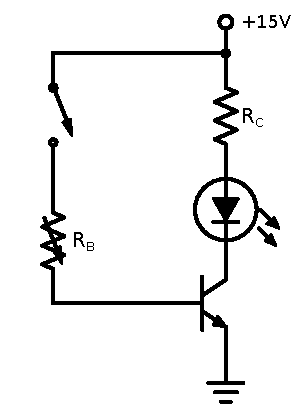
\includegraphics[width=35mm]{cc1.pdf}
	\label{fig:cc1}
\end{wrapfigure}

\subsection{interruttore semplice}
Utilizzando la breadboard come sostegno abbiamo realizzato il circuito riportato in Fig. \ref{fig:cc1}; sono stati utilizzati inoltre un transistor BC107B, un LED verde, una resistenza nominale da $\SI{1}{\kilo\ohm}$ ($R_C =(9991 \pm 2) \si{\ohm}$) e una decade di resistenze. La decade di resistenza è stata inizialmente settata a $\SI{100}{\kilo\ohm}$ ($R_B = (99.902 \pm 0.003)\si{\kilo\ohm}$).
Una volta alimentato il circuito assemblato, abbiamo notato il LED accendersi. In tale situazione il generatore di corrente continua forniva una corrente di \SI{13}{\milli\ampere}. Aprendo il circuito, invece, il LED si spegneva. Ciò è dovuto al fatto che tra base ed emettitore, essendoci una giunzione p-n, è necessario avere almeno una $V_{BE}=0.6 \si{\volt}$. Nel caso dell'interruttore aperto, come vediamo dallo schema del circuito, non abbiamo più una differenza di potenziale tra base ed emettitore e dunque il transistor risulta interdetto. 

Per studiare il range in cui il transistor può lavorare come interruttore e dove invece entra in saturazione, abbiamo collegato in serie alla decade di resistenze un amperometro, in modo tale da sapere la corrente $I_B$ che circolava in quel ramo del circuito. Avendo a disposizione quindi sia la corrente totale $I_{tot}$ (dato fornito dal generatore), che la corrente $I_B$ abbiamo potuto ricavare la corrente di collettore $I_C$, la stessa da cui era attraversato il LED.
\begin{equation*}
	I_{tot} = I_B + I_C \quad \rightarrow \quad I_C = I_{tot} - I_B
\end{equation*}


\begin{wrapfigure}[22]{r}[0pt]{125mm}
	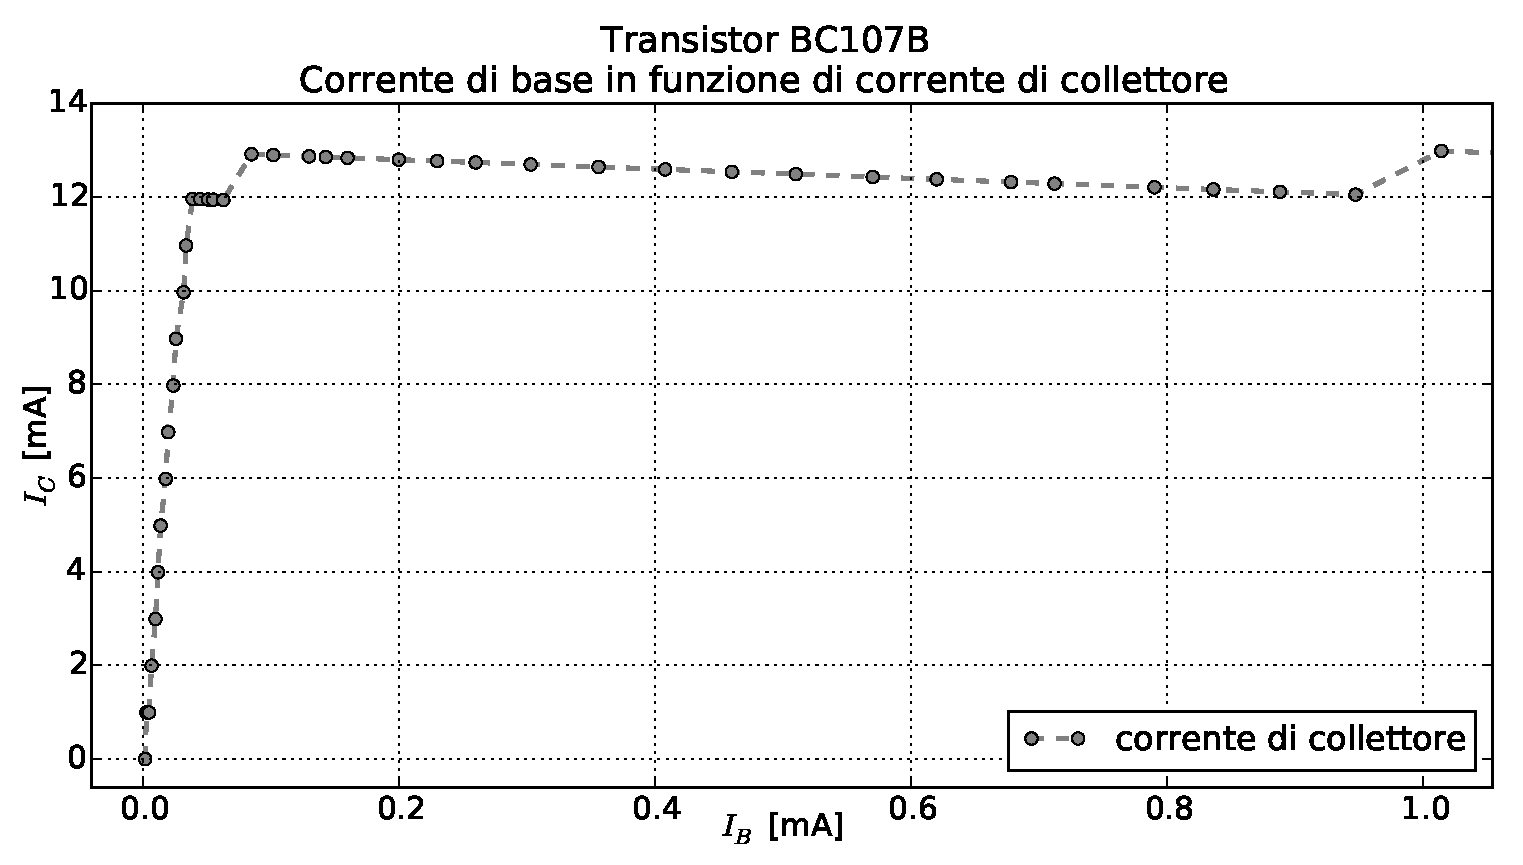
\includegraphics[width=125mm]{saturazione_2.pdf}
	\caption{I grafico mostra la corrente da cui è percorso il diodo in funzione della corrente di base. I dati per $I_B \geq 1.05$ non sono mostrati perché poco significativi.}
	\label{fig:saturazione}
\end{wrapfigure}

Variando il valore di resistenza $R_B$ della decade abbiamo ottenuto un set di dati che correlava $I_B$ a $I_C$.
Il problema di questo metodo è la risoluzione del dato di corrente fornito dal generatore.
Esso infatti non ha un numero di cifre significative uguale a quello dell'amperometro.
Nonostante questa problematica, gli strumenti a nostra disposizione sono stati sufficienti per ricavare approssimativamente un range di lavoro per il transistor.

%%%	- questo grafico è la versione con tutti i dati - %%%
%\begin{wrapfigure}[18]{r}[0pt]{120mm}
%	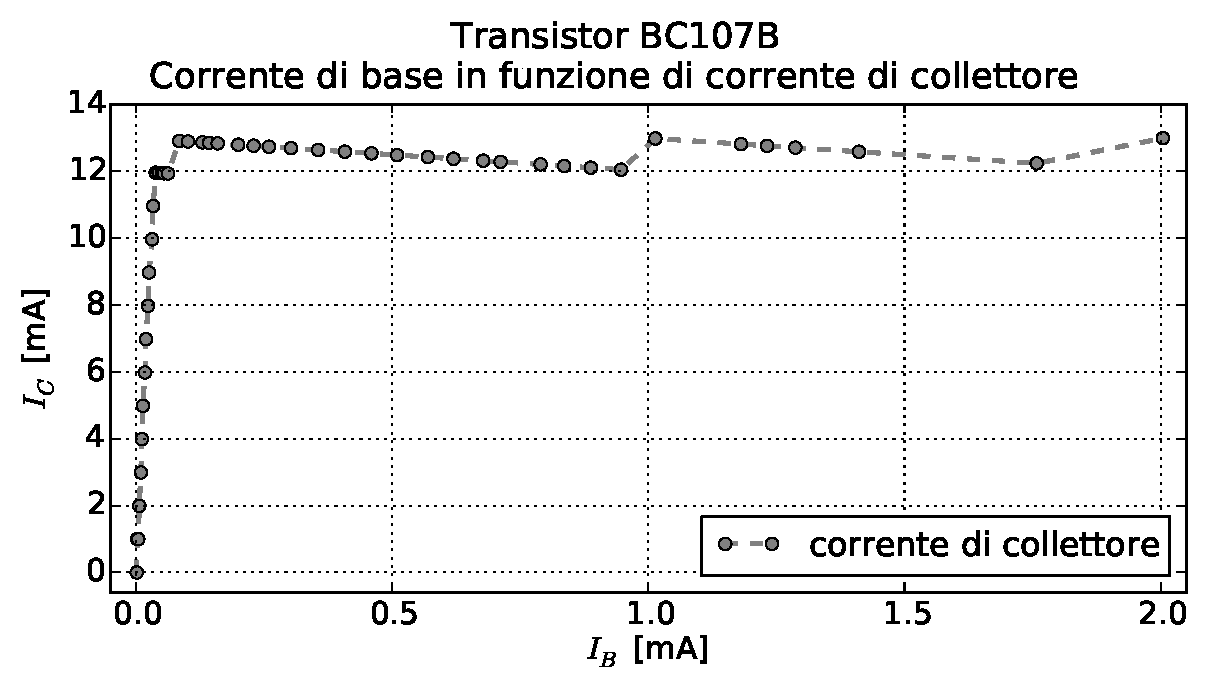
\includegraphics[width=120mm]{saturazione.pdf}
%	\caption{I grafico mostra la corrente da cui è percorso il diodo in funzione della corrente di base.}
%	\label{fig:saturazione}
%\end{wrapfigure}

%%%	- questo grafico è la versione con i dati compresi tra 0 e 1.05- %%%

Dai dati graficati in Fig. \ref{fig:saturazione} abbiamo dedotto che il range di lavoro del transistor è lineare per $I_B \leq \SI{40}{\micro\ampere}$, mentre per $I_B \geq \SI{100}{\micro\ampere}$ il transistor è sicuramente in saturazione. Nel range in cui il transistor non è in saturazione è possibile usare la decade di resistenze come ''potenziometro`` per comandare l'intensità della luce emessa dal LED.
\newpage
\begin{wrapfigure}[13]{r}[0pt]{35mm}
	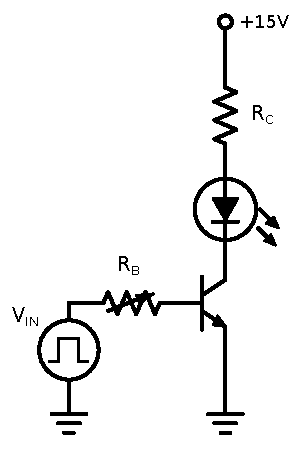
\includegraphics[width=35mm]{cc2.pdf}
	\caption{Transistor come interruttore veloce.}
	\label{fig:cc2}
\end{wrapfigure}
\subsection{interruttore veloce}
Per questa parte dell'esperienza abbiamo montato il circuito mostrato in Fig. \ref{fig:cc2}.
La decade è stata settata a \SI{10}{\kilo\ohm} ($R_B = (9993 \pm 2)\si{\ohm}$), mentre la resistenza $R_C$ è rimasta la stessa del circuito precedente.
Il circuito è stato infine alimentato con un'onda quadra ad una frequenza compresa nel range $10-100\,\si{\hertz}$. %il valore di R_B l'ho inventato!%

È stata poi condotta un'analisi puramente qualitativa sul funzionamento dell'interruttore. Abbiamo osservato che impostando la frequenza dell'onda quadra ad un valore di pochi \si{\hertz} si notava il lampeggio del LED. Aumentando gradualmente la frequenza si faceva sempre più difficoltà a percepire lo sfarfallio della luce emessa, fino ad una frequenza di circa \SI{55}{\hertz}, da noi dichiarata come frequenza limite, cioè la frequenza a cui non si nota più lo sfarfallio, ma si osserva una luce accesa.

Utilizzando però lo stratagemma di avvicinare il viso al circuito e fissare un oggetto poco distante in modo da includere il LED nel proprio campo di visione periferico, siamo riusciti a notare nuovamente lo sfarfallio della luce emessa. La frequenza limite in queste condizioni si è alzata a circa \SI{65}{\hertz}